\documentclass[border=8pt]{standalone}
\usepackage{pgfplots}
\pgfplotsset{compat=1.18}
\providecommand{\pk}{red!75!black}
\begin{document}
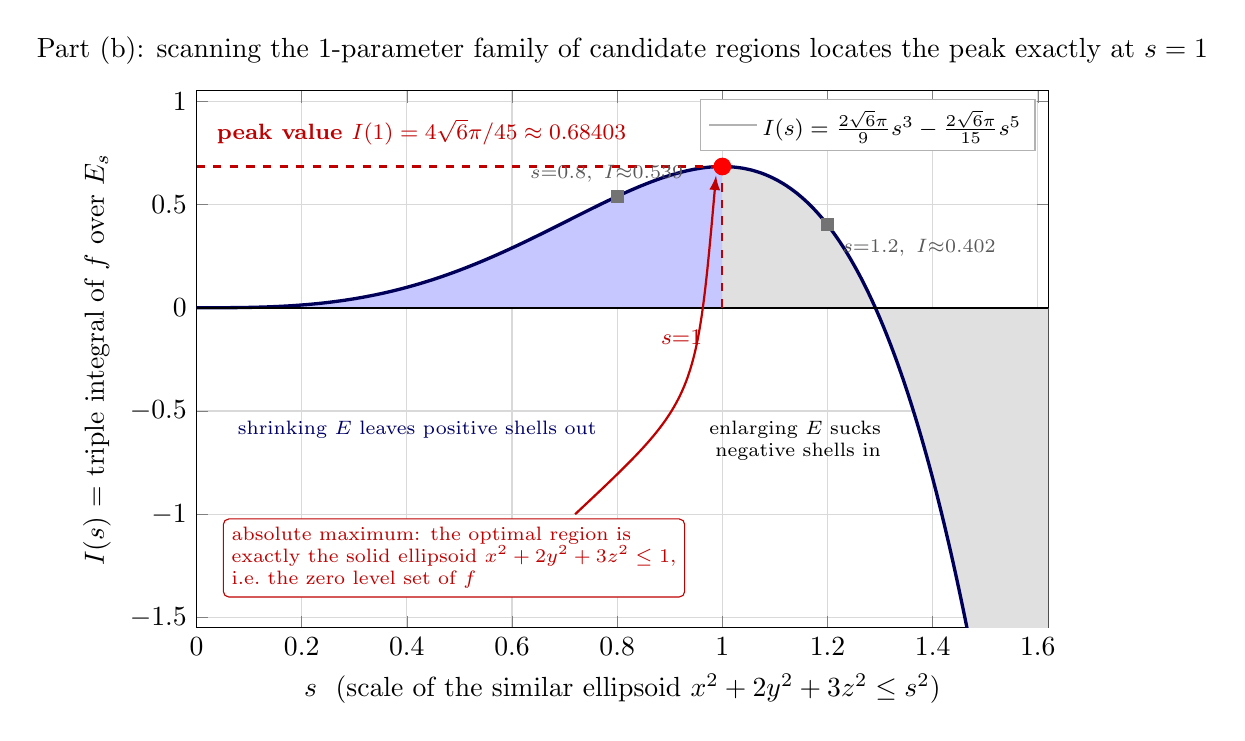
\begin{tikzpicture}
\begin{axis}[
    width  = 12.4cm, height = 8.4cm,
    xmin=0, xmax=1.62, ymin=-1.55, ymax=1.05,
    xlabel={$s$ \ (scale of the similar ellipsoid $x^2+2y^2+3z^2\le s^2$)},
    ylabel={$I(s)$ = triple integral of $f$ over $E_s$},
    title={Part (b): scanning the 1-parameter family of candidate regions
           locates the peak exactly at $s=1$},
    every title/.append style={font=\small, align=center},
    grid=major, grid style={black!15},
    legend style={at={(0.985,0.985)}, anchor=north east, fill=white, draw=black!30,
                  font=\footnotesize},
    clip mode=individual,
]
% ---- shaded "too small / too large" zones --------------------------------
\addplot[fill=blue!22, draw=none, domain=0:1, samples=101] {15.390866*(x^3/9 - x^5/15)} \closedcycle;
\addplot[fill=black!12, draw=none, domain=1:1.62, samples=101] {15.390866*(x^3/9 - x^5/15)} \closedcycle;

% ---- the curve I(s) = (2 sqrt6 pi/9) s^3 - (2 sqrt6 pi/15) s^5 ------------
\addplot[very thick, blue!35!black, domain=0:1.62, samples=401]
    ({x}, {15.390866*(x^3/9 - x^5/15)});

% ---- zero axis ------------------------------------------------------------
\addplot[black, thick] coordinates {(0,0) (1.62,0)};

% ---- peak markers ---------------------------------------------------------
\addplot[\pk, thick, dashed] coordinates {(1,0) (1,0.6840266)};
\addplot[\pk, thick, dashed] coordinates {(0,0.6840266) (1,0.6840266)};
\addplot[only marks, mark=*, mark size=3pt, red] coordinates {(1,0.6840266)};
\node[\pk, font=\footnotesize\bfseries, anchor=north east] at (axis cs:0.98,-0.06) {$s{=}1$};
\node[\pk, font=\footnotesize\bfseries, anchor=south west] at (axis cs:0.02,0.74)
     {peak value $I(1)=4\sqrt6\pi/45\approx0.68403$};

% ---- callout --------------------------------------------------------------
\node[\pk, font=\scriptsize, align=left, inner sep=3pt, draw=\pk,
      fill=white, rounded corners=2pt, anchor=north west] at (axis cs:0.05,-1.02)
      {absolute maximum: the optimal region is\\
       exactly the solid ellipsoid $x^2+2y^2+3z^2\le 1$,\\
       i.e.\ the zero level set of $f$};
\draw[-latex, \pk, thick] (axis cs:0.72,-1.00) .. controls (axis cs:0.95,-0.45) ..
      (axis cs:0.988,0.640);

% ---- sample points --------------------------------------------------------
\addplot[only marks, mark=square*, mark size=2.2pt, black!55] coordinates {(0.8,0.5393) (1.2,0.4019)};
\node[black!65, font=\scriptsize, anchor=south] at (axis cs:0.78,0.56) {$s{=}0.8,\ I{\approx}0.539$};
\node[black!65, font=\scriptsize, anchor=north west] at (axis cs:1.21,0.38) {$s{=}1.2,\ I{\approx}0.402$};

% ---- zone captions --------------------------------------------------------
\node[blue!40!black, font=\scriptsize, anchor=north west] at (axis cs:0.06,-0.50)
     {shrinking $E$ leaves positive shells out};
\node[black, font=\scriptsize, align=right, anchor=north east] at (axis cs:1.32,-0.50)
     {enlarging $E$ sucks\\ negative shells in};

\addlegendentry{$I(s)=\frac{2\sqrt6\pi}{9}s^3-\frac{2\sqrt6\pi}{15}s^5$};
\end{axis}
\end{tikzpicture}
\end{document}
